\section{Speckle y procesamiento}

\subsection{Speckle}

\begin{frame}{} \vskip0cm
  \begin{figure}
    \centering
    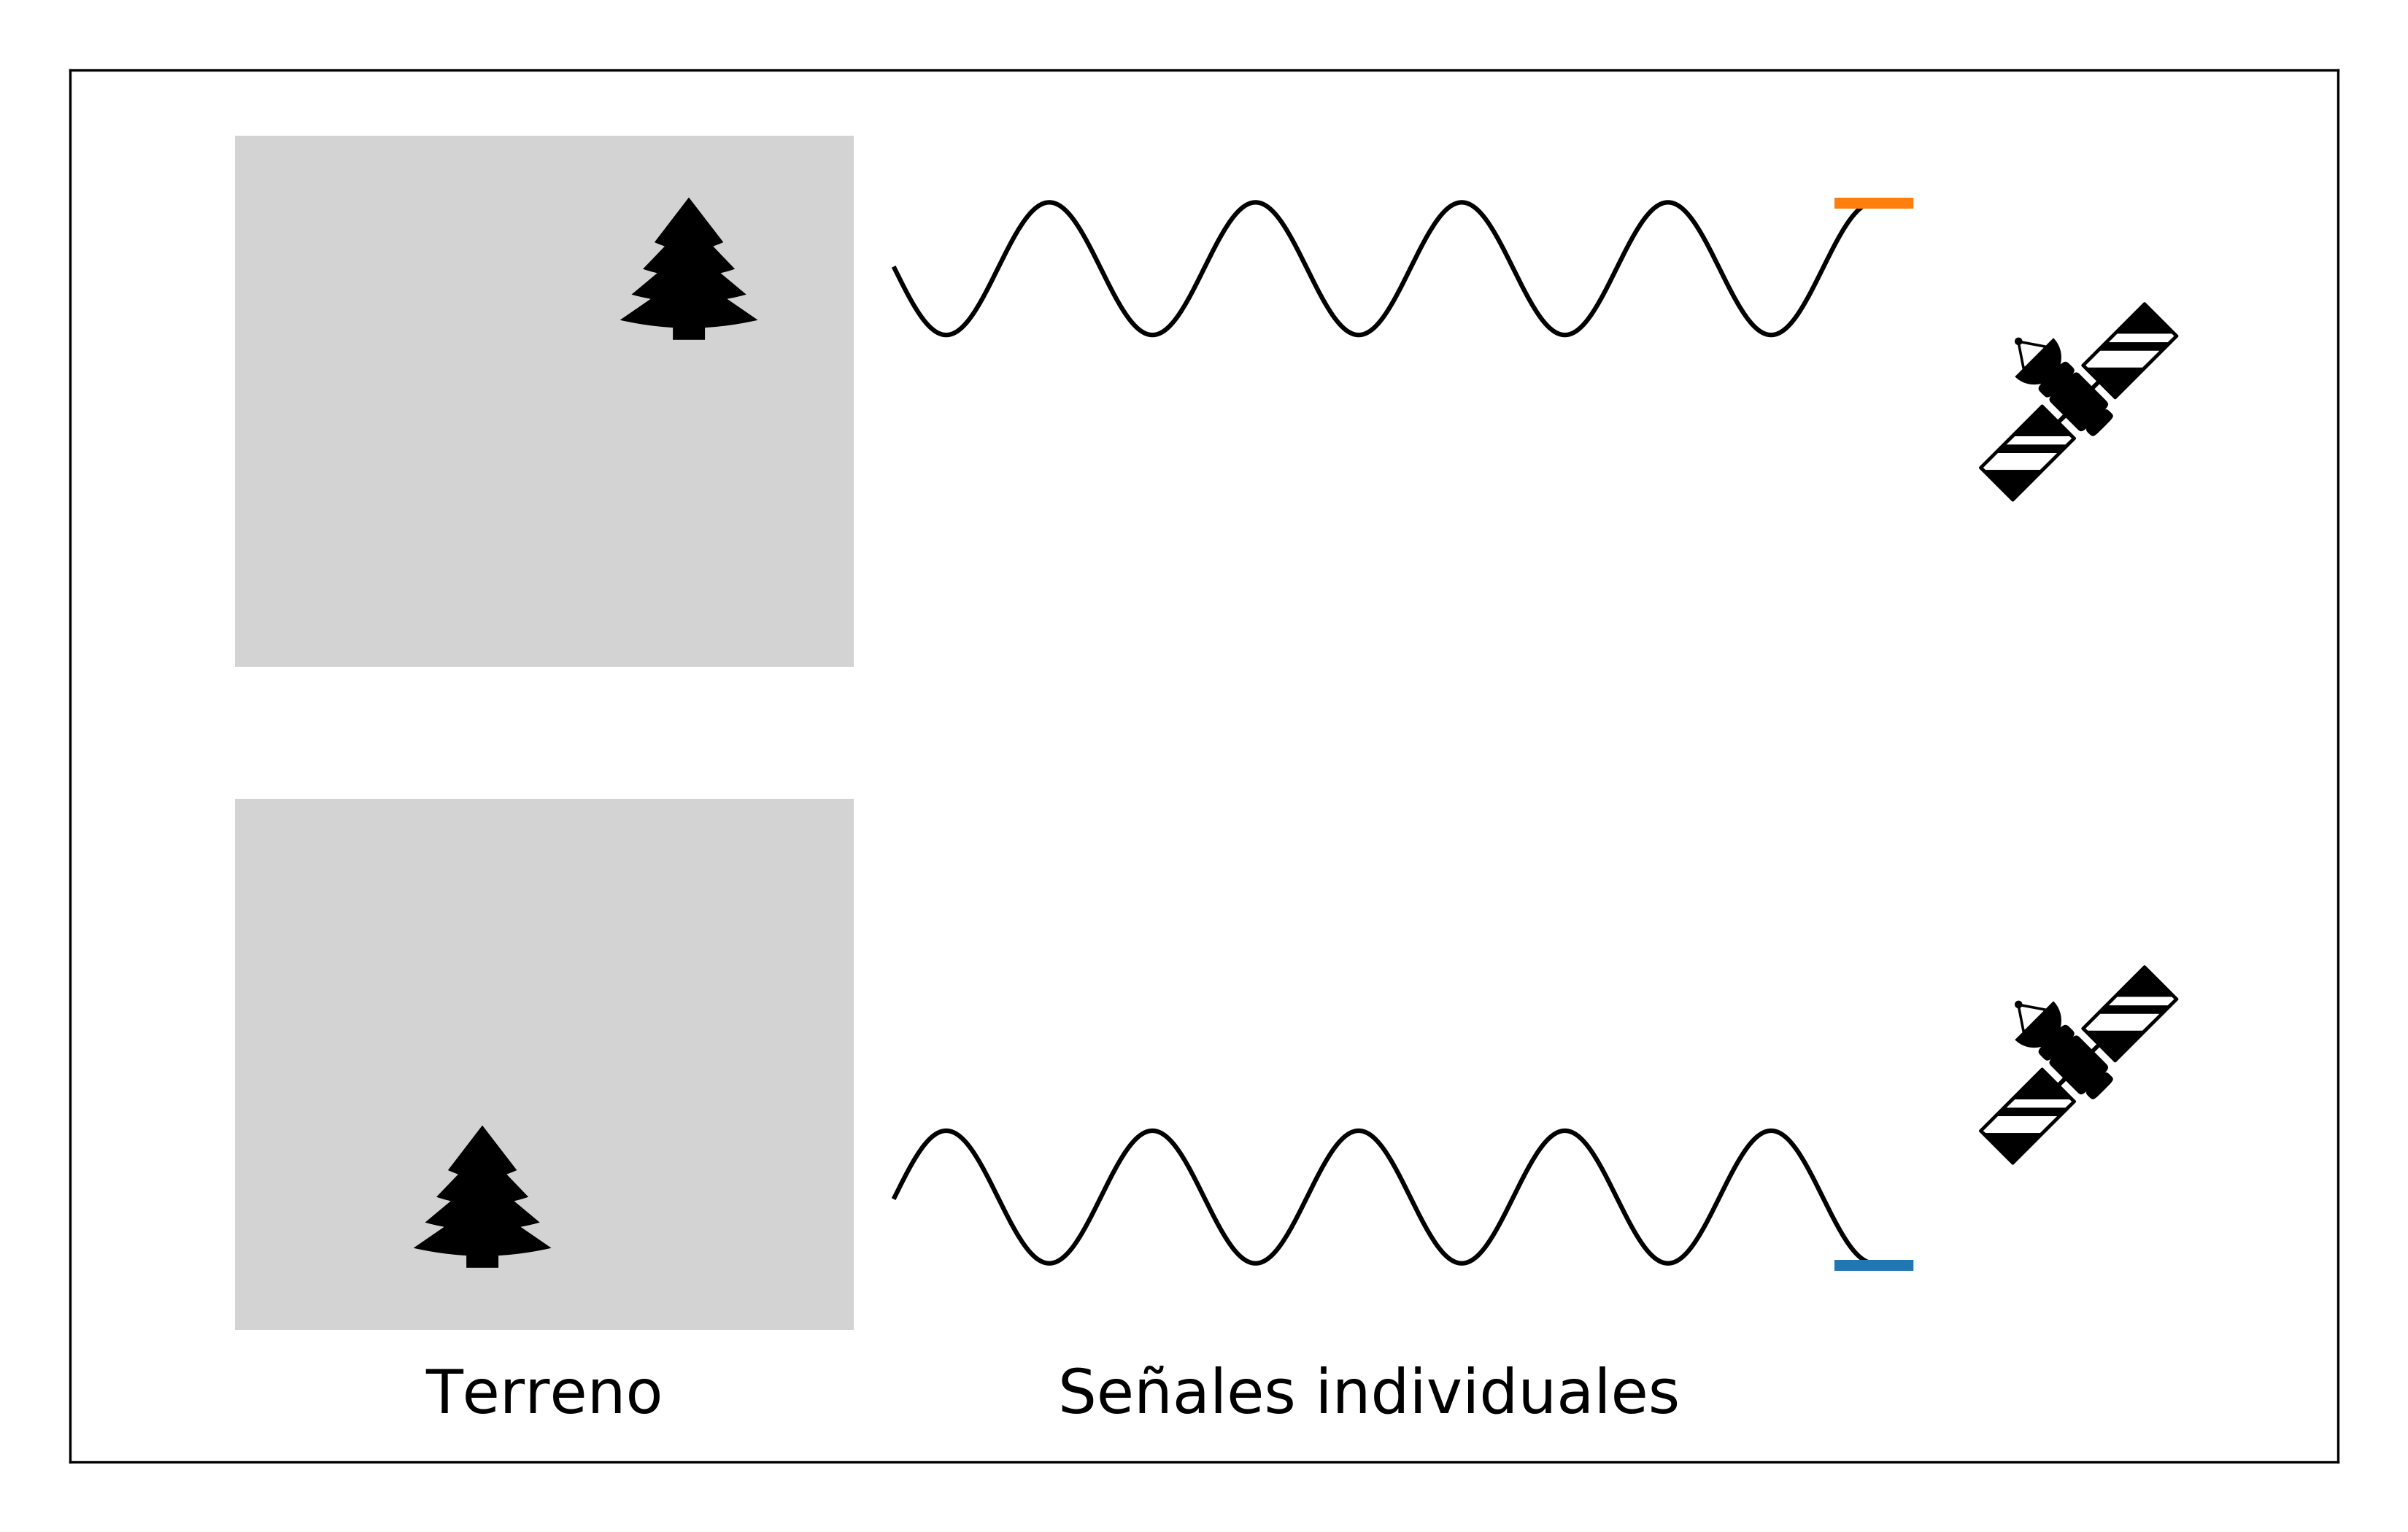
\includegraphics[width=0.65\textwidth]{fig:fase.png}
    \caption{Medición de fase y amplitud para un solo blanco.}
    \label{}
  \end{figure}
\end{frame}
%--- Next Frame ---%

\begin{frame}{} \vskip0cm
  \begin{figure}
    \centering
    \movie[width = 0.95\textwidth,loop,autostart]{\centering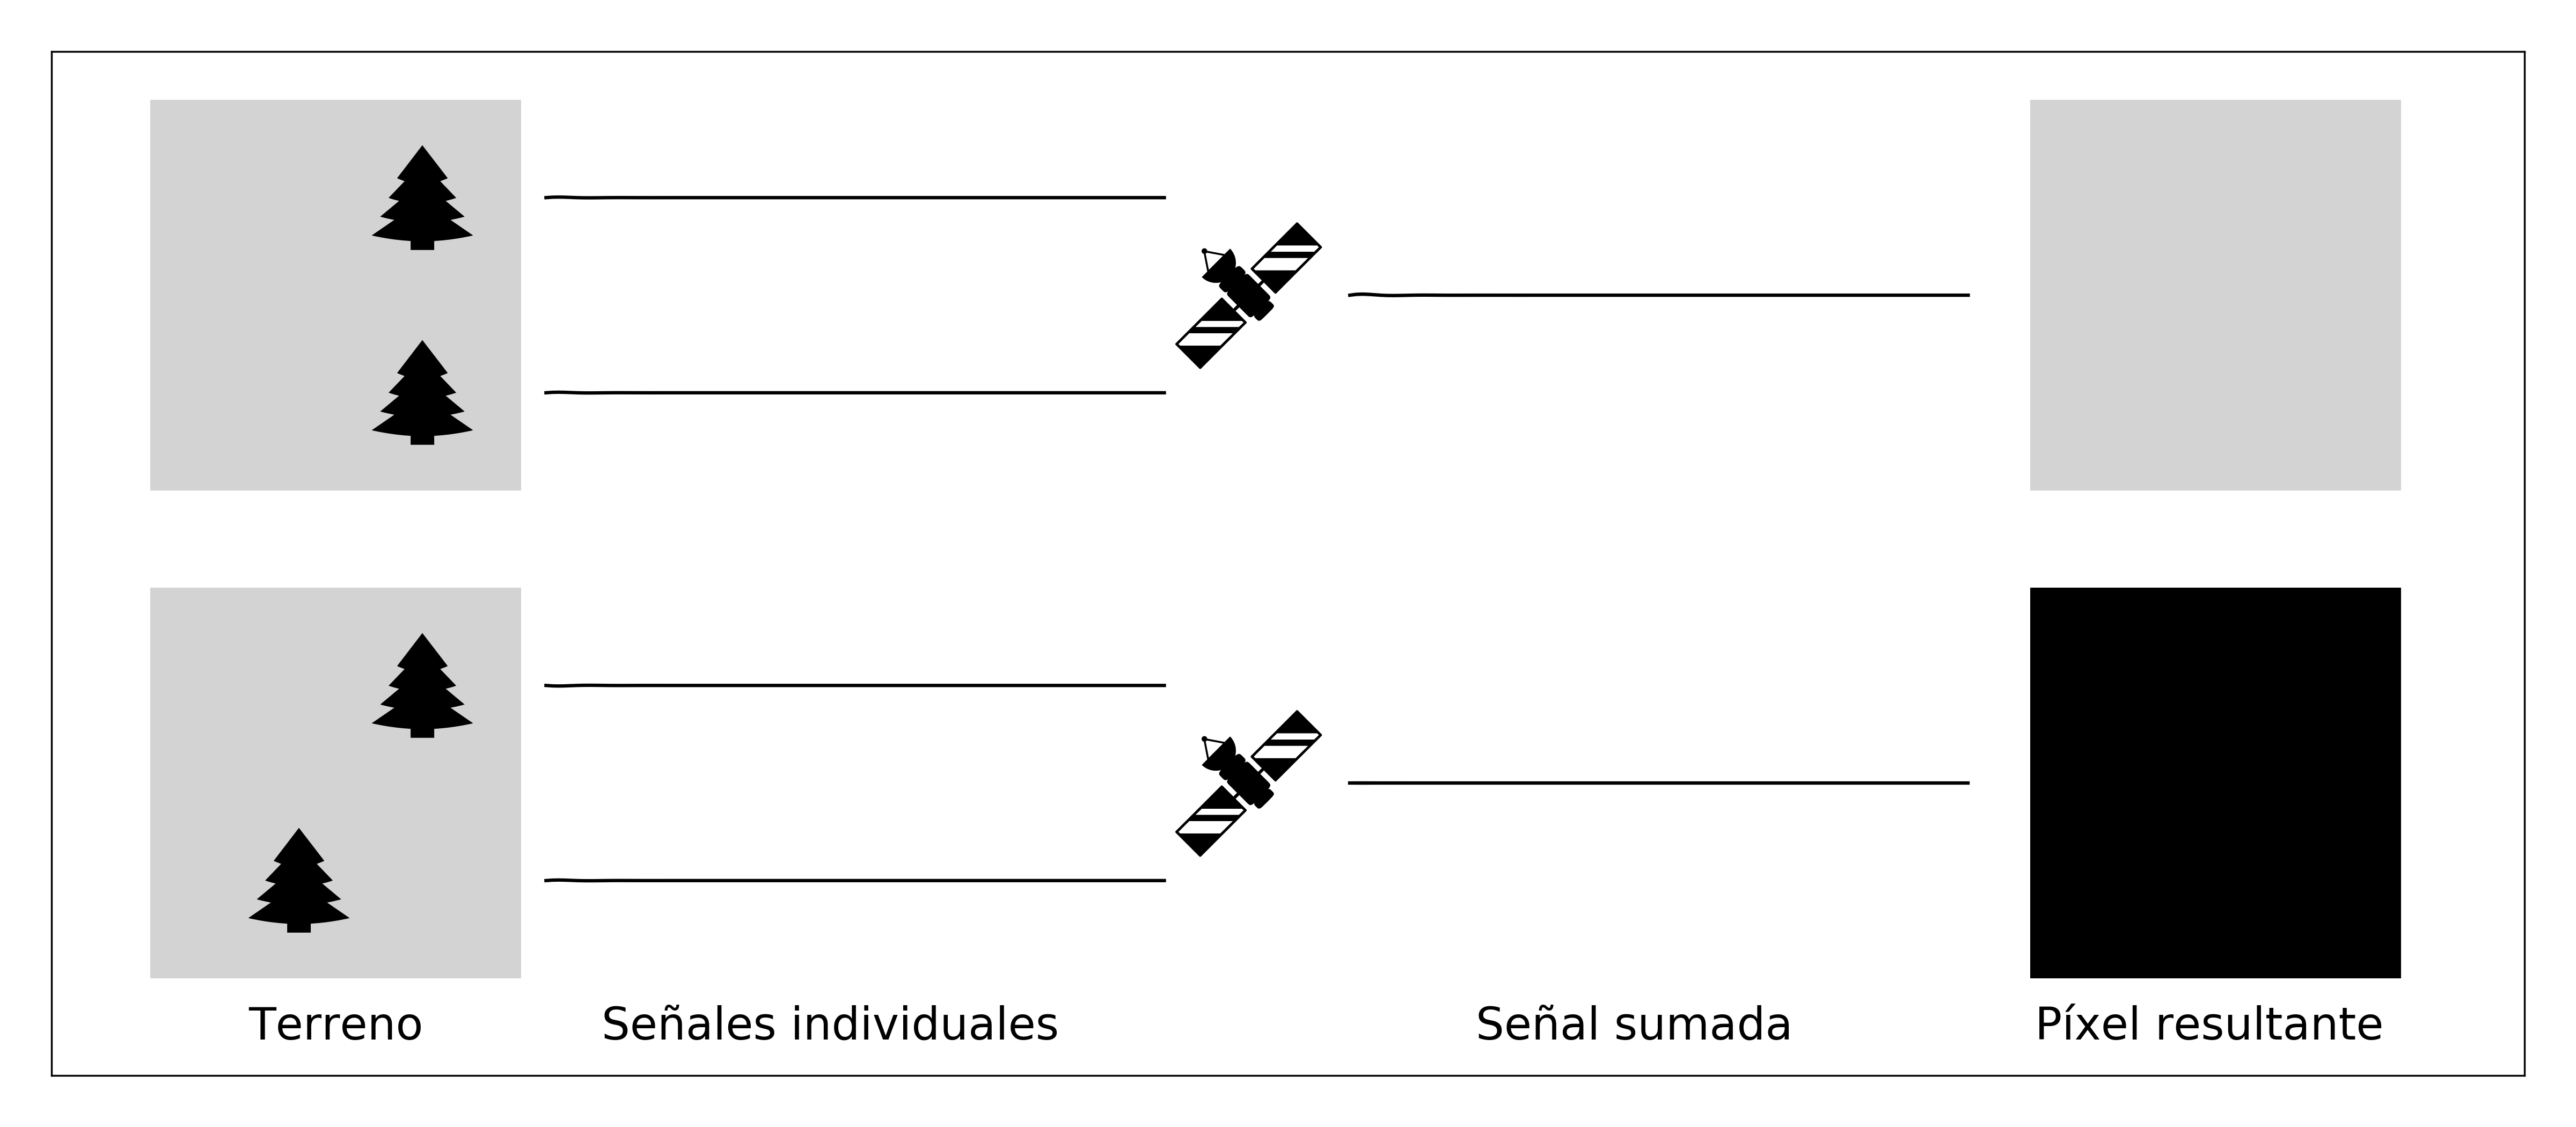
\includegraphics[width=0.95\textwidth]{fig:speckle.png}}{./figs/fig:speckle.mp4}
    \caption{Medición de fase y amplitud con varios blancos dentro del píxel.}
    \label{}
  \end{figure}
\end{frame}
%--- Next Frame ---%


\begin{frame}{} \vskip0cm
  \begin{itemize}
    \item El specke no es ruido, es determinístico. Si repito la adquisición manteniendo la geometría el patrón de specke resulta idéntico.
    \item Si promedio dos pixeles en amplitud tendré el mismo problema. Tengo que promediarlos en potencia (multilooking)
  \end{itemize}
      \begin{figure}
        \centering
        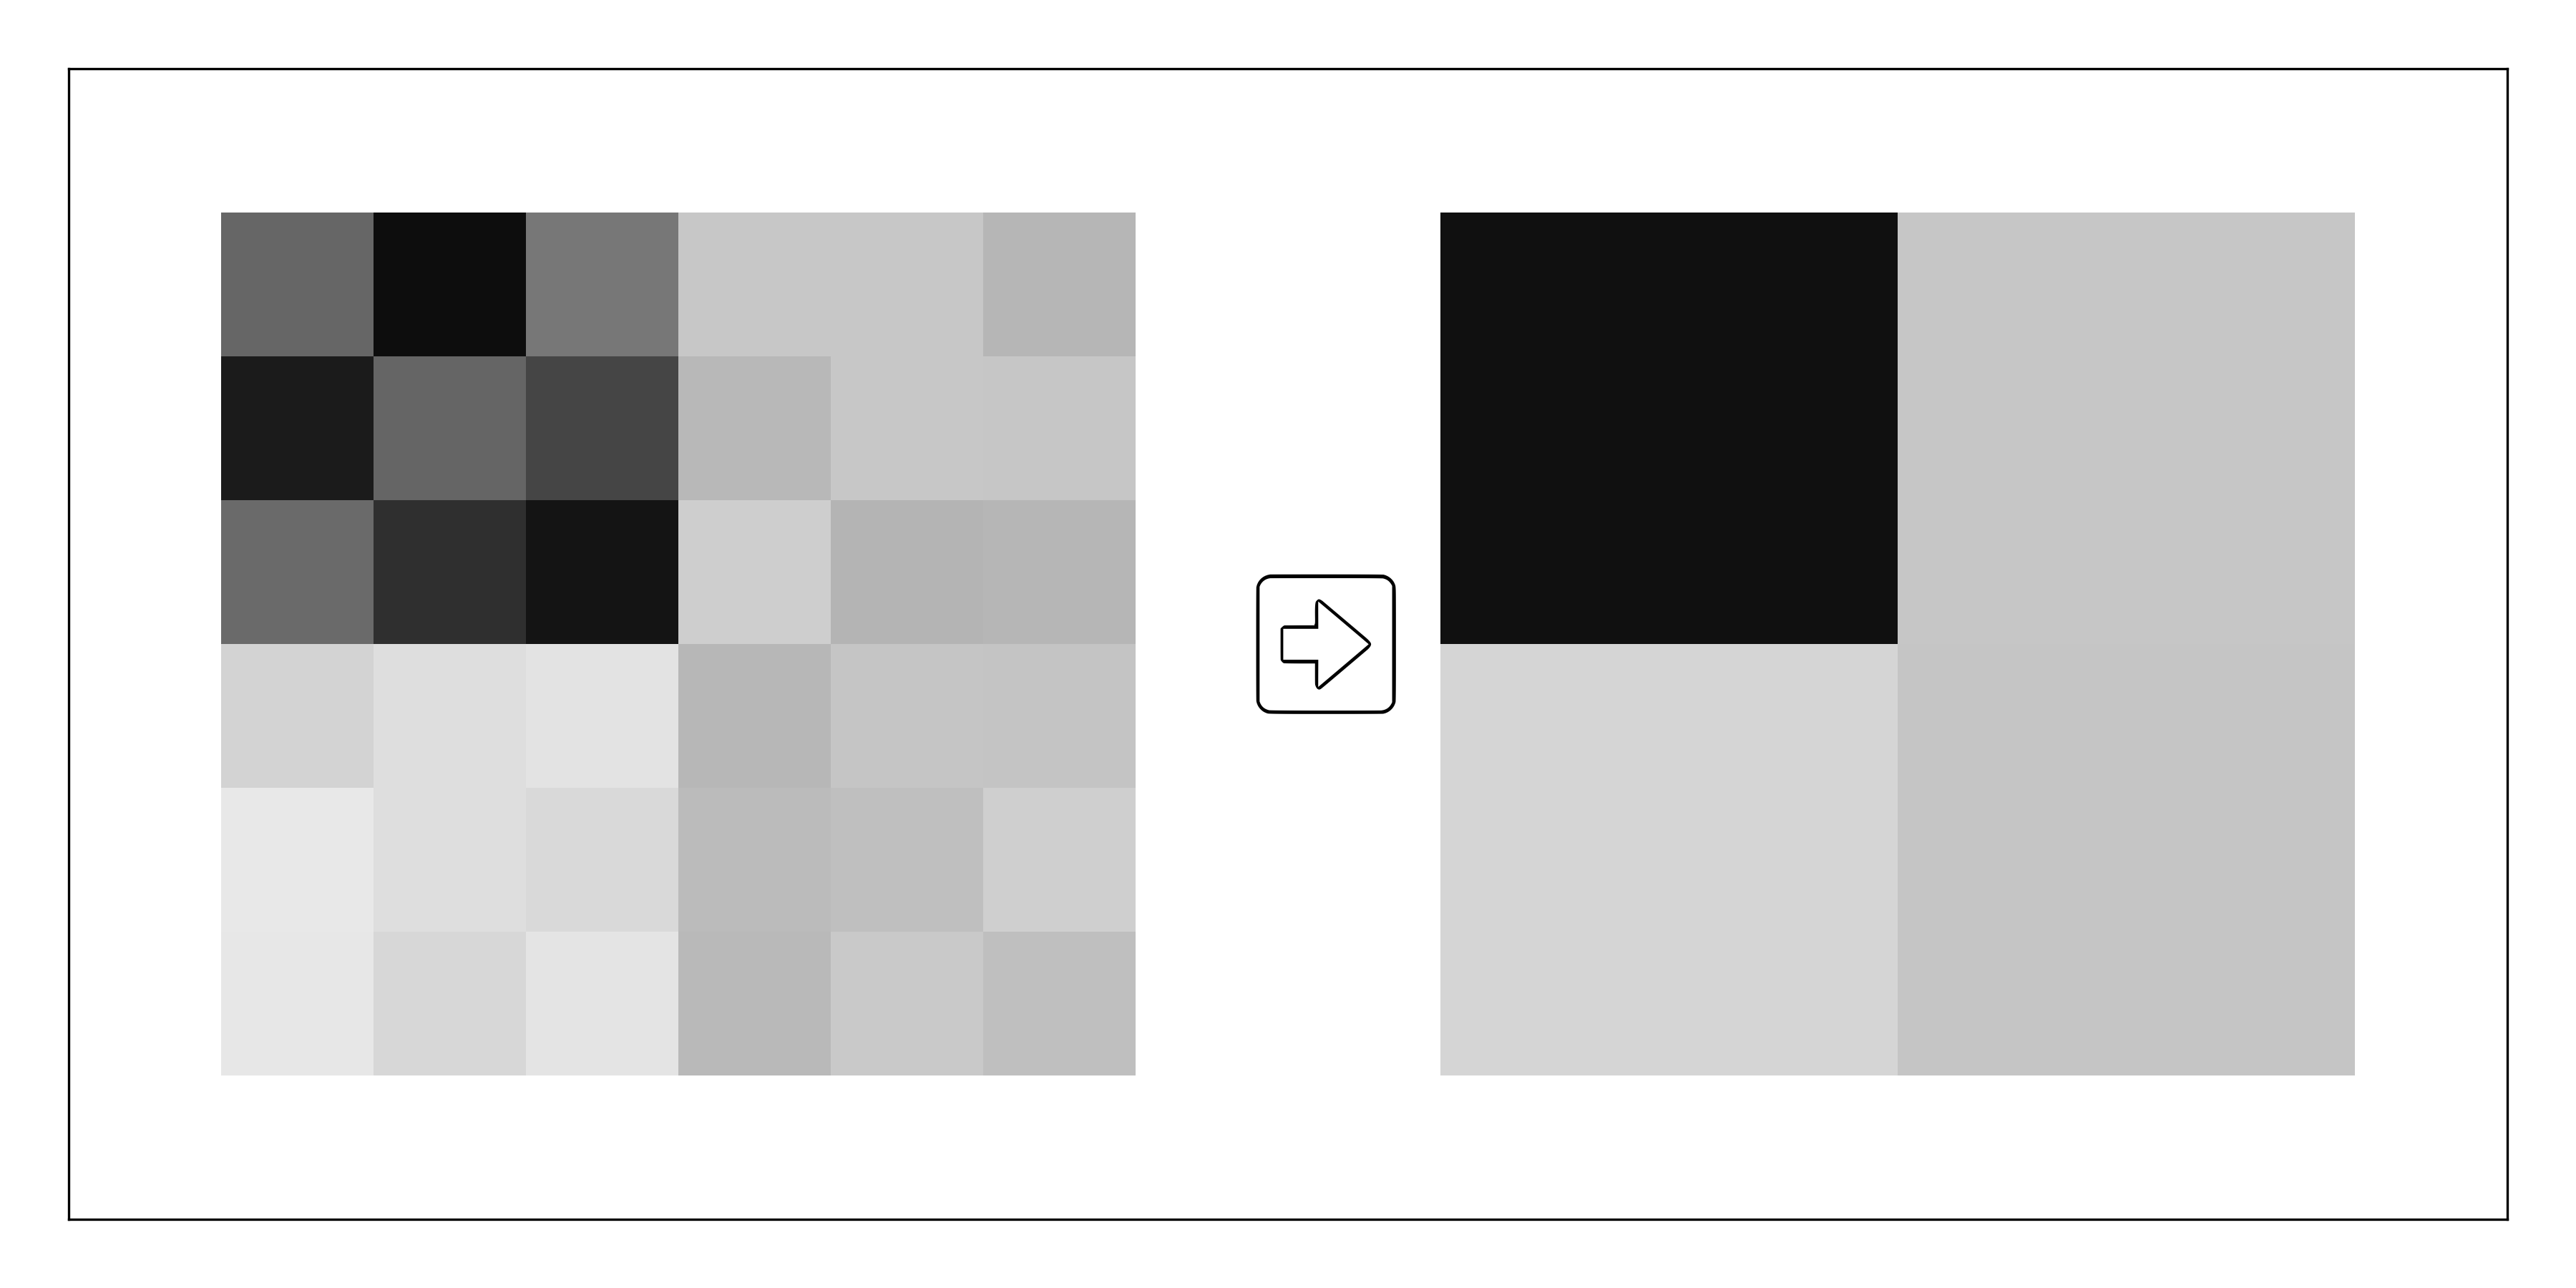
\includegraphics[width=0.65\textwidth]{fig:multilook.png}
        %\caption{Proceso de multilook.}
        \label{}
      \end{figure}

\end{frame}
%--- Next Frame ---%


\begin{frame}{} \vskip0cm

   \begin{block}{Multilook}
     \begin{itemize}
       \item Se promedian en potencia varios píxeles vecinos y se los asigna a uno nuevo
       \item Se pierde resolución.
       \item Efectivo contra el speckle.
     \end{itemize}
   \end{block}

\end{frame}
%--- Next Frame ---%

\begin{frame}{} \vskip0cm
  \begin{columns}
  \begin{column}{0.5\textwidth}
    \begin{figure}
      \centering
      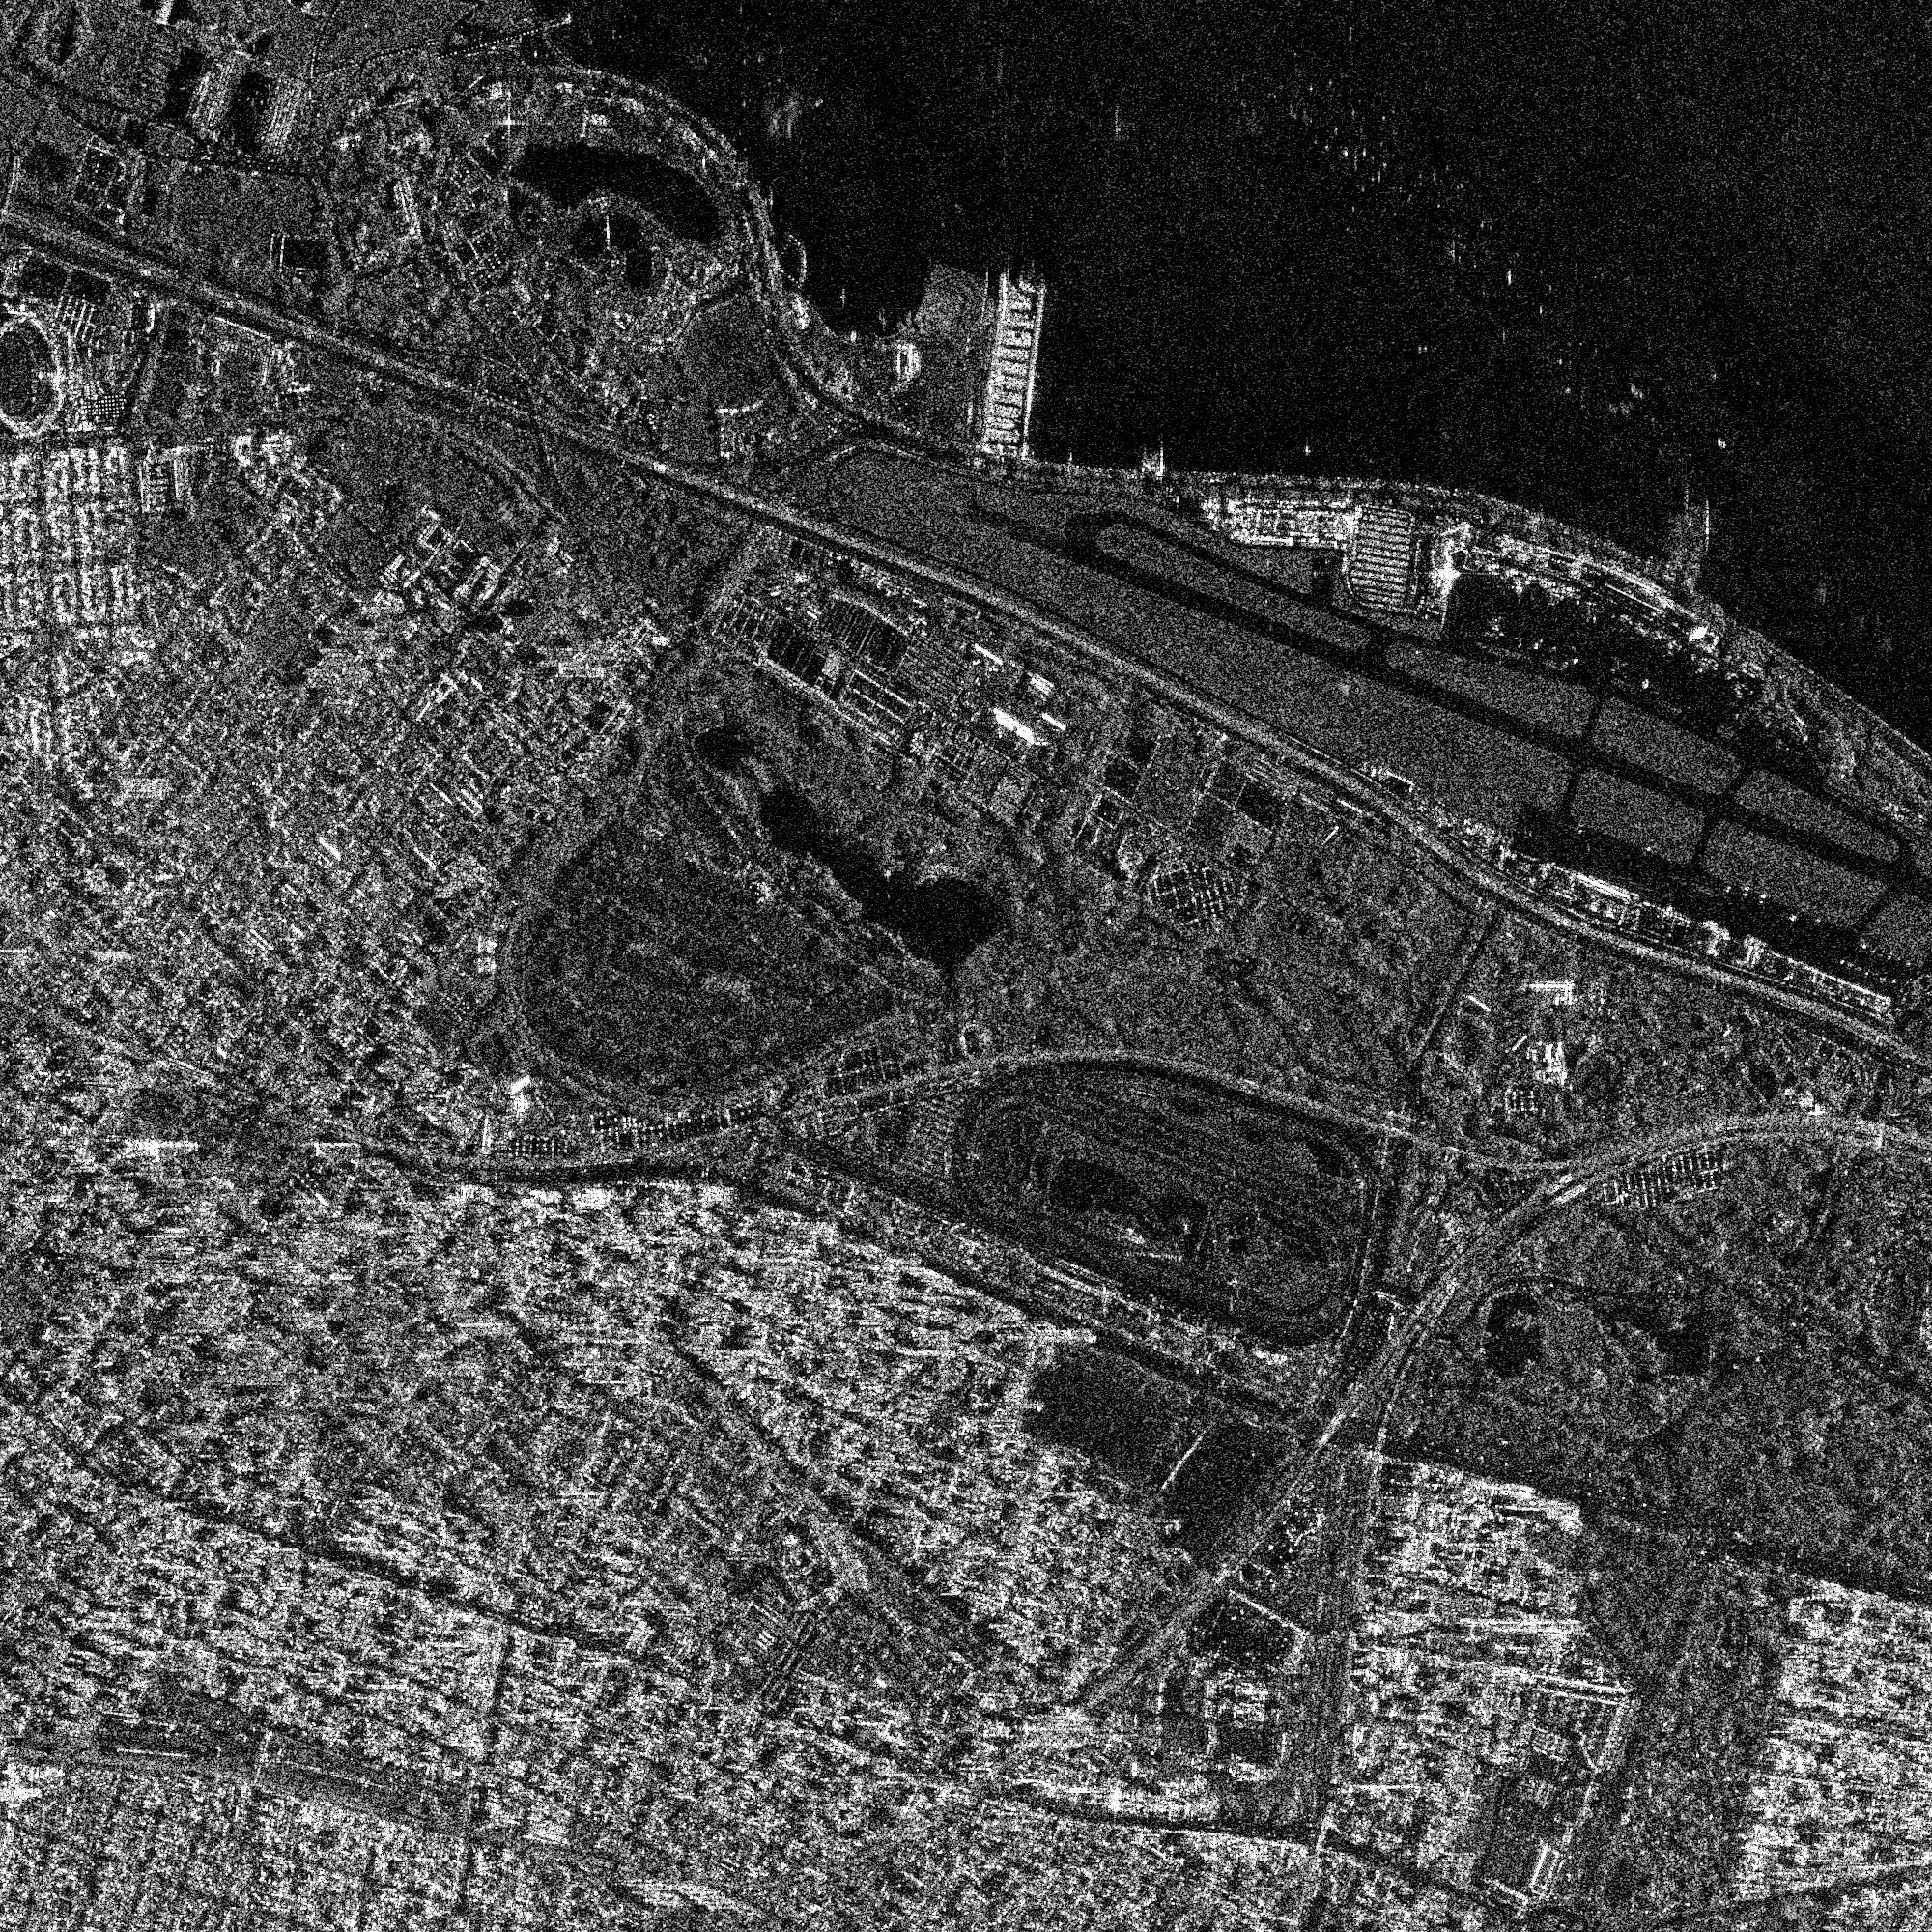
\includegraphics[width=0.8\textwidth]{fig:original.jpg}
      \caption{Imagen original.}
      \label{}
    \end{figure}
  \end{column}
  \begin{column}{0.5\textwidth}  %%<--- here
    \begin{figure}
      \centering
      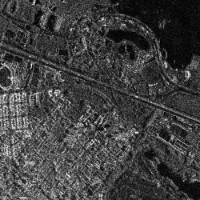
\includegraphics[width=0.8\textwidth]{fig:multilook.jpg}
      \caption{Imagen multilookeada.}
      \label{}
    \end{figure}
  \end{column}
  \end{columns}
\end{frame}
%--- Next Frame ---%


\subsection{Distorciones geométricas}

\begin{frame}{} \vskip0cm
      \begin{figure}
        \centering
        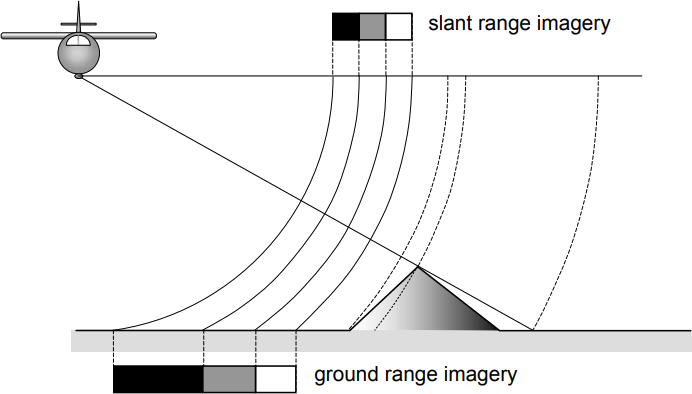
\includegraphics[width=0.8\textwidth]{fig:slant.png}
        \caption{Comparación entre Slant range y Ground range.}
        \label{}
      \end{figure}
\end{frame}
%--- Next Frame ---%

\begin{frame}{} \vskip0cm
      \begin{figure}
        \centering
        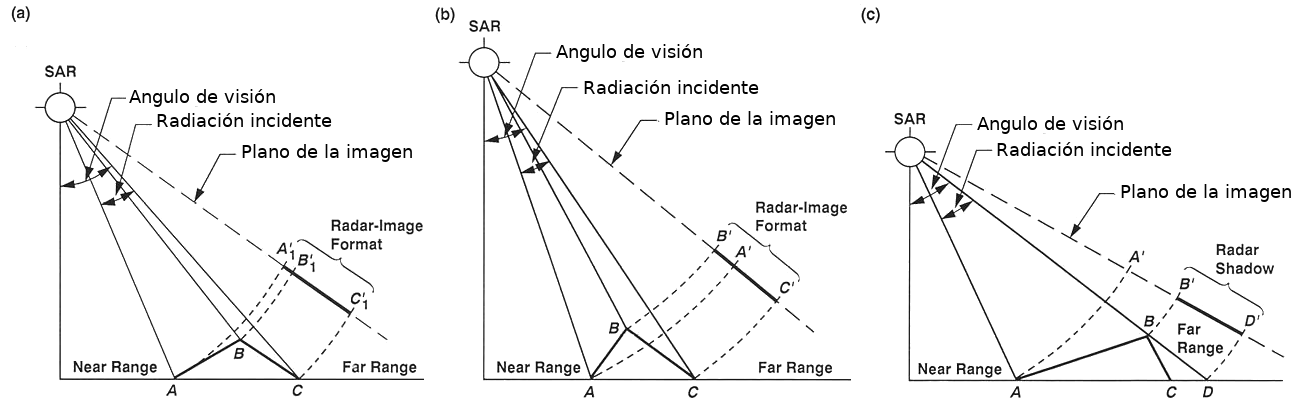
\includegraphics[width=\textwidth]{fig:dist.png}
        \caption{Distorciones geométricas típicas en una imagen radar:\\ {\centering a. foreshortening, b. layover, c. shadowing.}}
        \label{}
      \end{figure}
\end{frame}
%--- Next Frame ---%

\begin{frame}{} \vskip0cm
    \begin{figure}
      \centering
      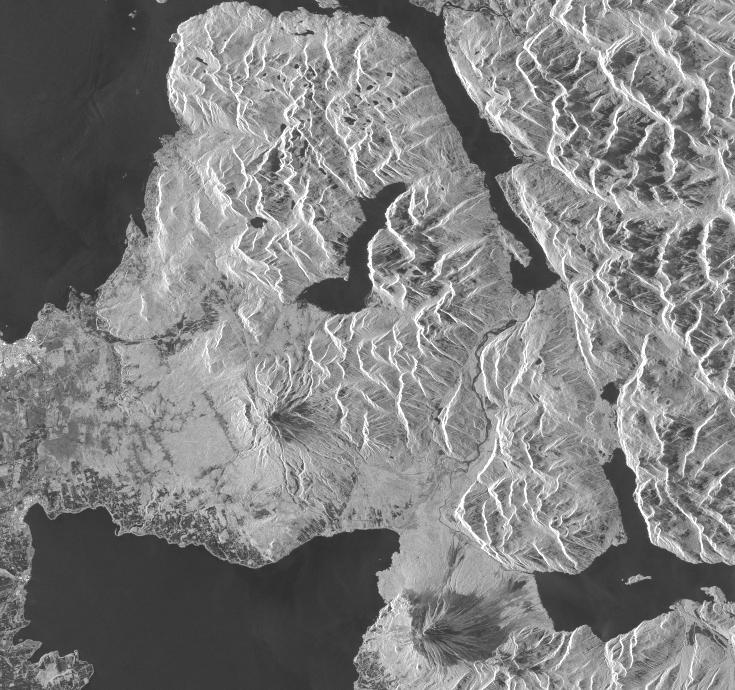
\includegraphics[width=0.5\textwidth]{fig:dist2.jpg}
      \caption{Vista de una imagen radar sin correcciones geométricas.}
      \label{}
    \end{figure}
\end{frame}
%--- Next Frame ---%

\begin{frame}{} \vskip0cm
  \begin{block}{Correcciones geométricas}
    Para resolver parte de las distorciones geométricas es util pasar la imagen del \emph{slant range} al \emph{ground range}. Para esto deberemos proyectarla y podemos hacerlo de dos maneras
    \begin{itemize}
      \item Sobre el elipsoide.
      \item Sobre un modélo de elevación digital.
    \end{itemize}
  \end{block}
\end{frame}
%--- Next Frame --- %

\subsection{Niveles de procesamiento}
\begin{frame}{} \vskip0cm
  % Please add the following required packages to your document preamble:
  % \usepackage{booktabs}
  % \usepackage{graphicx}
  \begin{table}[]
  \centering
  \resizebox{\textwidth}{!}{%
  \begin{tabular}{@{}cccc@{}}
  \toprule
  L1A (SLC)                                                                                                    & L1B (GRD)                                                                  & L1C (GEC)                                                                              & L1D (GTC)                                                                                     \\ \midrule
  Single Look Complex                                                                                          & Ground Range Detected                                                      & Geocoded Elipsoid Corrected                                                            & Geocoded Terrain Corrected                                                                    \\
  \multicolumn{1}{p{4.5cm}}{Datos en formato complejo (real e imaginario), sin multilook y en la geometria del radar} & \multicolumn{1}{p{4.5cm}}{Datos en potencia, con multilook y proyectada al suelo} & \multicolumn{1}{p{4.5cm}}{Datos en potencia, con multilook y geocodificada sobe el elipsoide} & \multicolumn{1}{p{4.5cm}}{Datos en potencia, con multilook y geocodificada sobe el el terreno (DEM)}\\
    \multicolumn{1}{p{4.5cm}}{
\includegraphics[width=4.3cm]{fig:l1a.png}} & \multicolumn{1}{p{4.5cm}}{
\includegraphics[width=4.3cm]{fig:l1b.png}} & \multicolumn{1}{p{4.5cm}}{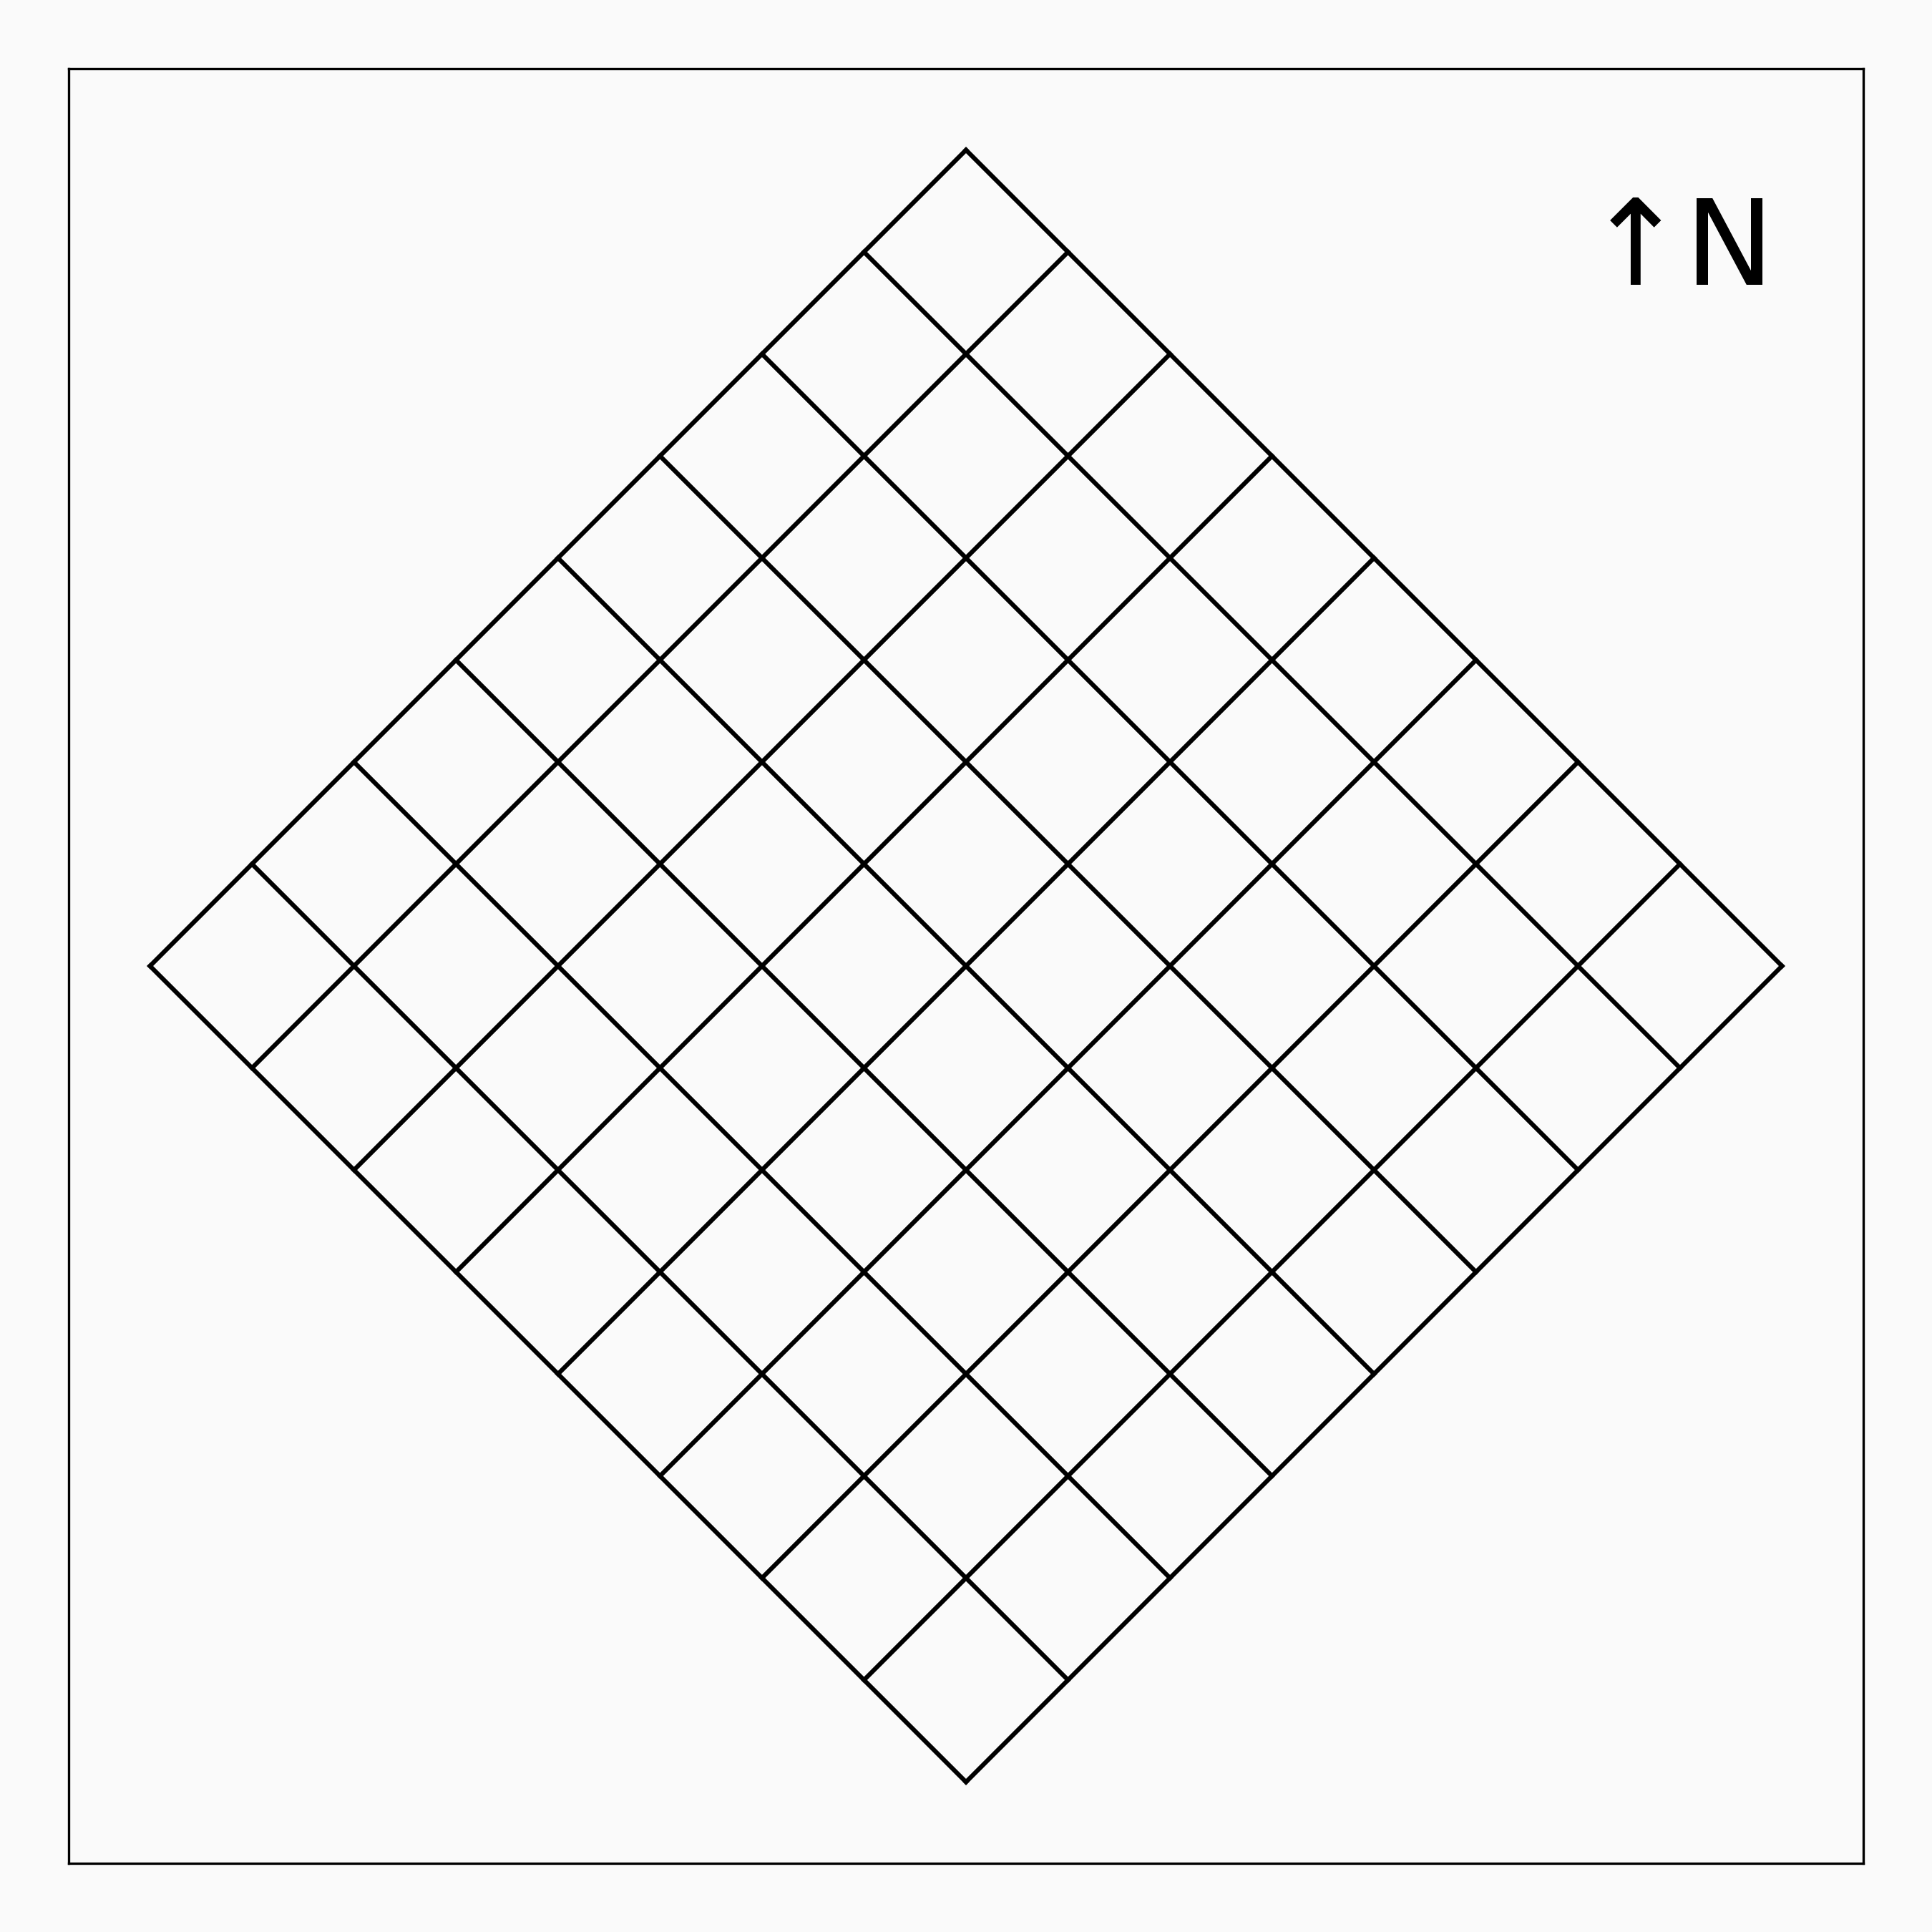
\includegraphics[width=4.3cm]{fig:l1c.png}} & \multicolumn{1}{p{4.5cm}}{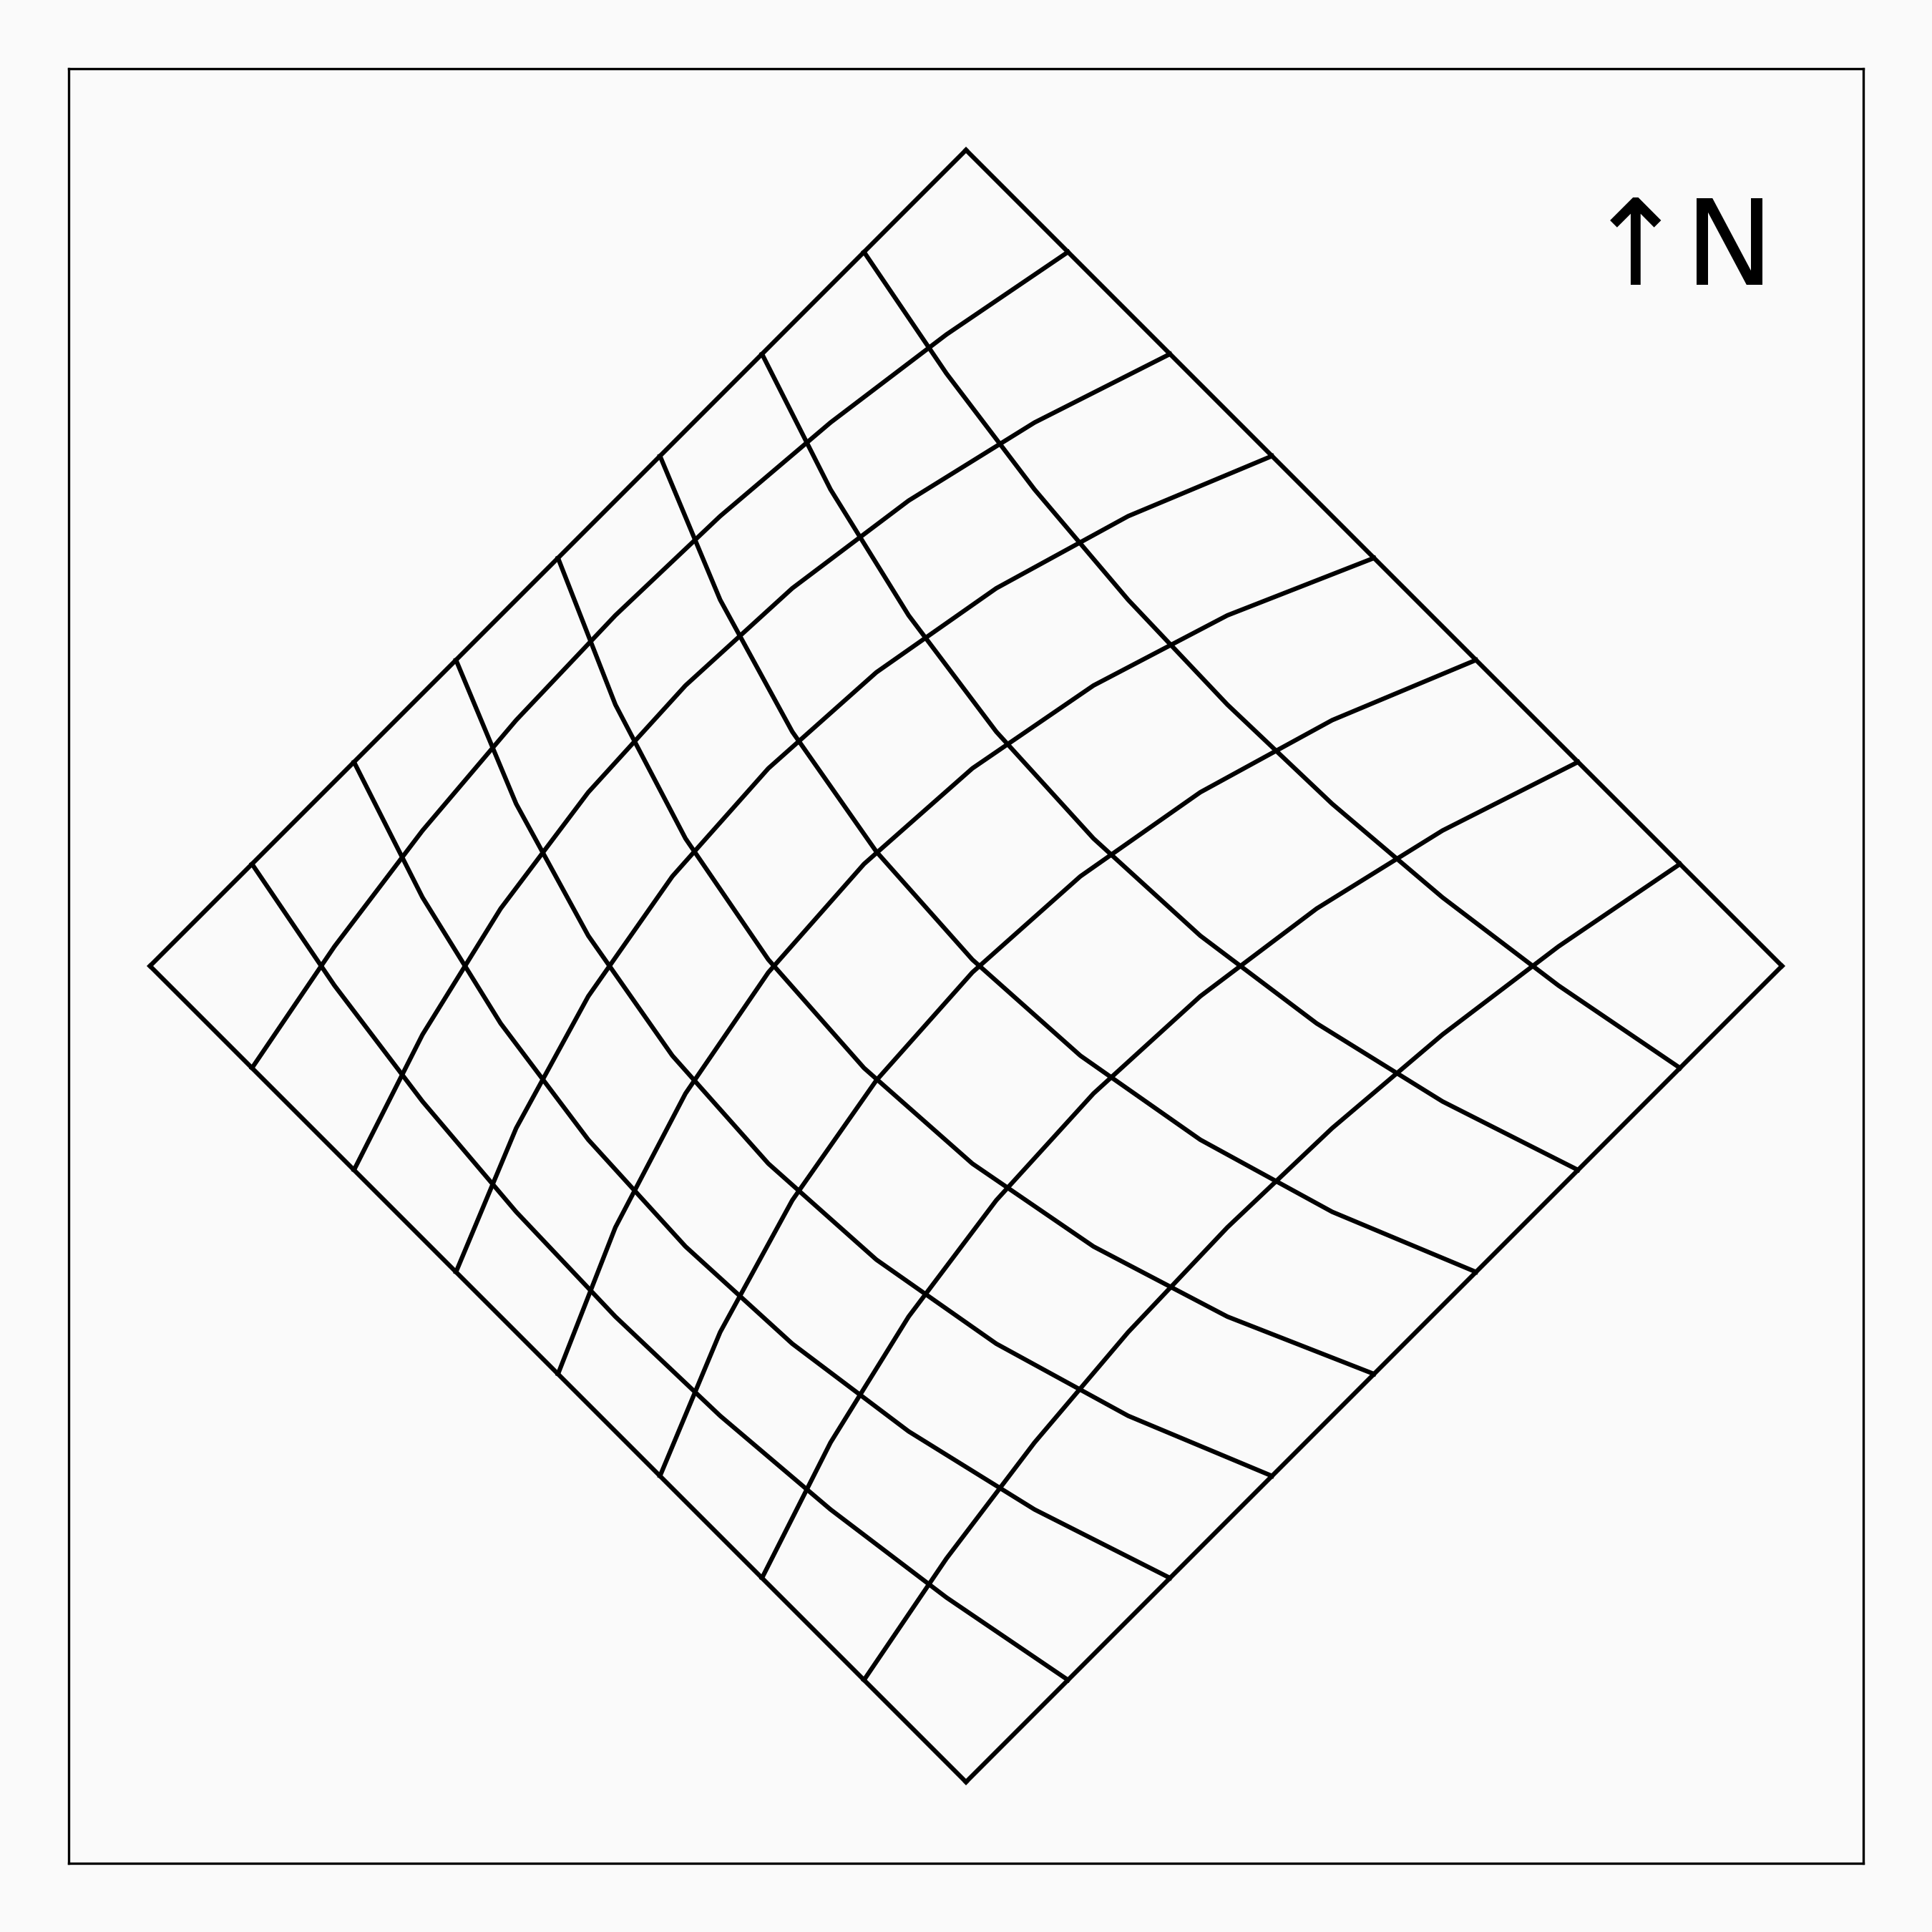
\includegraphics[width=4.3cm]{fig:l1d.png}}\\
    \bottomrule
  \end{tabular}%
  }
  \caption{Niveles de procesamiento típicos para una imagen SAR.}
  \label{my-label}
  \end{table}
\end{frame}

\gracias
%--- Next Frame ---%
